\documentclass[a4paper, amsfonts, amssymb, amsmath, reprint, showkeys, nofootinbib, twoside]{revtex4-1}
\usepackage[english]{babel}
\usepackage[utf8]{inputenc}
\usepackage[colorinlistoftodos, color=green!40, prependcaption]{todonotes}
\usepackage[pdftex, pdftitle={Article}, pdfauthor={Author}]{hyperref} % For hyperlinks in the PDF
\usepackage{graphicx} % For figures
\usepackage{algorithm} % For algorithms
\usepackage{algpseudocode}

%\setlength{\marginparwidth}{2.5cm}
\bibliographystyle{apsrev4-1}
\begin{document}
\title{Self-Organization in the Minority Game}

\author{Gaëtan Ecrepont}
    \email[]{gaetan.ecrepont@polytechnique.edu}
    \affiliation{ENS Paris-Saclay, FRANCE}
\author{Guillaume Martin-Festa}
    \email[]{guillaume.martin-festa@polytechnique.edu}
    \affiliation{ENS Paris-Saclay, FRANCE}

\date{\today} % Leave empty to omit a date

\begin{abstract}
    We explore the Minority Game, a repeated binary prediction game introduced by Challet and Zhang which exhibits emergent behaviors revolving around the idea of self-organization. After an overview of the game and its dynamics, we empirically study its volatility and predictability under various configurations, highlighting the existence of a phase transition between two distinct regimes. Finally, we recast the Minority Game in the context of financial markets and discuss the implications of our findings in this context. In particular, we argue that financial markets exhibit self-organized criticality and thus operate at the edge of efficiency.
\end{abstract}


\maketitle

This paper is organized into four sections. In Section \ref{sec:introduction}, we first introduce the El Farol Bar problem and then move on to the Minority Game, which is motivated by the former. In Section \ref{sec:presentation}, we present the theoretical framework of the Minority Game and then derive its dynamics. In Section \ref{sec:self-organization}, we study the two key emergent behaviors of the system: volatility and predictability. Finally, in Section \ref{sec:financial-markets}, we link the Minority Game to financial markets and recast our findings in this context.


\section{Introduction}
\label{sec:introduction}

\subsection{El Farol Bar problem}
A key concept in strategic decision-making is \textit{inductive thinking}, which can be roughly described as the ability to learn from the past to make inferences about the future. It is very different from \textit{deductive thinking}, which amounts to applying a predefined set of rules to a given situation. A classic game-theoretic introduction to inductive thinking for decision-making is Brian Arthur's \textit{El Farol Bar problem} \cite{Arthur_1994}, which we present in this section.

The problem is simple: every Thursday, 100 people consider visiting the El Farol Bar, but the venue is enjoyable only if attendance stays below 50. If too many go, the bar is overcrowded; if too few go, those who stayed home may regret missing out. Without direct communication, individuals must predict attendance based on past data. If their forecast suggests a crowded bar, they stay home; otherwise, they go. Every night, individuals make their decision independently, and the bar's attendance fluctuates based on their choices.

To win this game, one needs to be in the \textit{minority}. Crucially, there is no single optimal strategy since the best decision depends on the decisions of others. This is a key feature of the game: agents must adapt to the behavior of others, leading to complex dynamics. The game is played repeatedly, and agents can learn from past experiences to improve their predictions.

To simulate this game using agent-based modelling, Arthur proposed that each agent uses a fixed set of simple forecasting rules (e.g. assuming attendance will be the same as last week or averaging past values). Over time, agents favor rules that perform well, adjusting their choices accordingly. Remarkably, Arthur's simulations showed that attendance naturally fluctuates around the optimal level of 50, despite the absence of central coordination. This \textit{self-organizing} behavior emerges from agents adapting to each other’s strategies through inductive thinking, without explicit communication or coordination.

There is more to be said about the El Farol Bar problem, but we will not go into details here. The key result is that \textit{inductive thinking can lead to self-organization}.


\subsection{The Minority Game}

The El Farol Bar problem directly inspired the Minority Game, a simple model introduced by Challet and Zhang \cite{Challet_1997} to study self-organization in a repeated binary prediction game.

In the Minority Game, an odd number of agents repeatedly choose between two options (e.g., A or B, buy or sell, go or stay, etc.) The goal is to be in the minority group\footnote{There is always a strict minority since the number of agents is odd.}. The game is played in identical rounds, and each agent has a fixed individual set of strategies to choose from. These strategies can be thought of as simple rules or heuristics that guide the agents' decisions based on past outcomes. At the end of each round, the agents in the minority (i.e. those who chose the less popular option) are the winners, while those in the majority (i.e. those who chose the more popular option) are the losers. At the end of each round, all agents update their \textit{all} of their strategies based on the outcome of the round, regardless of which strategy they actually played\footnote{As we will see in the last section, rewarding strategies even though they weren't actually played amounts to neglecting one's impact on the aggregate outcome.}.

Just like the El Farol bar problem, this is a \textit{negative sum game} since by definition only the minority wins at each round. Ideally, agents would coordinate so that the minority is a large as it can be (i.e. half the population). And indeed computer simulations show that the game naturally \textit{self-organizes} to a state where the number of agents in the minority is close to half the population, though with fluctuations around this value.


\section{Presentation of the system}
\label{sec:presentation}

We now formally introduce the model. We first review the mathematical framework of the Minority Game before deriving its dynamics. This is only a brief presentation,, and for more details we refer the reader to the original paper by Challet and Zhang \cite{Challet_1997}.

\subsection{Theoretical framework}

Throughout the rest of the paper, we will use the following notations:
\begin{itemize}
    \item $N$: number of agents
    \item $S$: number of strategies per agent
    \item $M$: memory length of each
    \item $s_i(t)$: strategy of agent $i$ at time $t$
    \item $S_i$: set of strategies of agent $i$
    \item $a_i(t)$: action of agent $i$ at time $t$
    \item $A(t) = \sum_{i=1}^N a_i(t)$: aggregate movement of the population at time $t$, also called \textit{attendance} in analogy with the El Farol Bar problem
    \item $a(t)$: action of the population at time $t$, defined as $a(t) = \text{sign}A(t)$
\end{itemize}

The game has $N$ agents, each with memory length $M$. The game's history is represented by binary string $H$ which is initialized as a $M$-long string of random bits and to which we append a \texttt{0} bit (resp. \texttt{1}) when the action $a(t)$ is $-1$ (resp. $+1$) at the end of round $t$.

At a given time $t$, agents base their action $a_i(t)$ on the last $M$ values in the game's history, i.e. on the \textit{state} $\mu(t) = (H[t-M], \ldots, H[t-1])$, which is a binary string of length $M$ that encodes the last $M$ actions of the population. Each agent has a set of $S$ strategies, which are mappings $\{0, 1\}^M \to \{-1, +1\}$ that determine the agent's action based on the current state $\mu(t) \ in \{0, 1\}^M$. The strategies are fixed and do not change over time. Each agent's individual set of strategies is denoted $S_i$.

At each turn $t$, each agent $i$ picks amongs its strategies $S_i$ the strategy $s_i(t)$ which has been the fittest so far, choosing randomly in case of a tie. The fitness of a strategy $s$ is defined as the number of times it has been in the minority so far, i.e. $F_s(t) = \sum_{t' < t} \mathbf{1}_{s(\mu(t')) = -a(t')}$. The agent then plays the action $a_i(t) = s_i(t)(\mu(t))$. Once all agents have picked their action\footnote{Note that the order of play is irrelevant since the attendance is the same regardless of the order.}, the population's action is computed as $a(t) = \text{sign}A(t)$. Finally, each player updates the fitness of all its strategies, as if it had played all of them\footnote{In some variants of the Minority Game, agents take into account their impact by giving an extra fitness reward to the strategy which they actually played. Interestingly, accounting for self-impact in this simple way removes many of the emergent phenomena of the game.}. Finally, the history is updated by appending the action of the population $a(t)$ to the history $H$.

The above set of rules can be summarized by the following algorithm:
\begin{algorithm}
    \caption{Minority Game}
    \label{alg:minority-game}
    \begin{algorithmic}[1]
        \State Initialize $H \sim U(\{0, 1\} ^M)$
        \For{$t = 0$ to $T$}
            \State $\mu(t) = H[t-M:t]$
            \For{$i = 1$ to $N$}
                \State $s_i(t) = \arg\max_{s \in S_i} F_s(t)$
                \State $a_i(t) = s_i(t)(\mu(t))$
            \EndFor
            \State $A(t) = \sum_{i=1}^N a_i(t)$
            \State $a(t) = \text{sign}A(t)$
            \For{$i = 1$ to $N$}
                \For{$s \in S_i$}
                    \State $F_s(t+1) = F_s(t) + \mathbf{1}_ {s(\mu(t)) = -a(t)}$
                \EndFor
            \EndFor
            \State $H \gets H \cup \{a(t)\}$
        \EndFor
    \end{algorithmic}
\end{algorithm}


\subsection{Dynamics}
For the sake of simplicity and like many authors \cite{Challet_1997}, we will assume that $S=2$ i.e. agents only have two strategies, which we will denote $s_{i,+}$ and $s_{i,-}$ for convenience. Note that doing so does not change the qualitative behavior of the system, but it does simplify the notations and alleviates the computations. Accordingly, we introduce the following useful notations:
\begin{itemize}
    \item $D_i(t) = \frac{1}{2}\big(F_{s_{i,+}}(t) - F_{s_{i,-}}(t)\big)$: difference of fitness between the two strategies of agent $i$ at time $t$
    \item $a_{i,+}^\mu$: action of agent $i$ when playing strategy $s_{i,+}$ and the game's state is $\mu$. We define $a_{i,-}^\mu$ similarly.
    \item $\omega_i^\mu = \frac{1}{2}\big(a_{i,+}^\mu + a_{i,-}^\mu\big)$
    \item $\xi_i^\mu = \frac{1}{2}\big(a_{i,+}^\mu - a_{i,-}^\mu\big)$
    \item $\Omega^\mu = \sum_{i=1}^N \omega_i^\mu$: can be thought of as the polarization of the system in state $\mu$.
\end{itemize}

Using those notations, the strategy ($s_{i,+}$ or $s_{i,-}$) played by agent $i$ at time $t$ is given by the sign of $D_i(t)$, i.e.
\begin{equation}
\label{eq:strategy}
    s_i(t) = \text{sign}(D_i(t))
\end{equation}
Consequently, the action of agent $i$ at time $t$ is given by:
\begin{equation}
    a_i(t) = a_{i,s_i(t)}^{\mu(t)} = \omega_i^{\mu(t)} + s_i(t) \xi_i^{\mu(t)}
\end{equation}
From which we can rewrite the attendance:
\begin{equation}
    A(t) = \Omega^{\mu(t)} + \sum_{i=1}^N s_i(t) \xi_i^{\mu(t)}
\end{equation}
The difference of fitness thus evolves according to the following equation:
\begin{equation}
\label{eq:difference}
    D_i(t+1) = D_i(t) - \xi_i^{\mu(t)} \textnormal{sign }A(t)
\end{equation}
Combining \eqref{eq:strategy} and \eqref{eq:difference}, we can see that the dynamics of the system is governed by the following equation:
\begin{equation}
\label{eq:dynamics}
    D_i(t+1) = D_i(t) - \xi_i^{\mu(t)} \textnormal{sign }\bigg(\Omega^{\mu(t)} + \sum_{j=1}^N s_j(t) \xi_j^{\mu(t)}\bigg)
\end{equation}
These equations are sufficient to simulate the dynamics of the Minority Game. We will now move on to study the emergent behaviors of the system, which is the main focus of this paper.


\section{Self-organization}
\label{sec:self-organization}

Now that we have presented the dynamics of the Minority Game, we can study its emergent behaviors. The two quantities of interest will be the \textit{volatility} and the \textit{predictability} of the system. The volatility measures how well the system self-organizes, while the predictability measures how well agents can predict the attendance. We will show that the two quantities are related and that they both depend on the parameter $\alpha = \frac{2^M}{N}$, with a critical value $\alpha_c \simeq 0.34$ which separates two distinct regimes.

\subsection{Volatility}

We have already said that the game self-organizes to a state where the number of agents in the minority is close to half the population. In other words, after a while the attendance will naturally tend to fluctuate around zero: $A(t) \simeq_{t \gg 1} 0$. We are interested in the amplitude of the oscillations around zero since they essentially measure how well the system self-organizes. In other words, we want to measure the volatility of the system $\sigma^2 = \langle A^2(t) \rangle$ where $\langle \cdot \rangle$ denotes the average over time.

To begin with, note that for fully random agents (i.e. agents flipping coins at each step to decide their action), we have $a_i(t) \sim U(\{-1, +1\}) \ i.i.d.$ with mean $0$ and variance $1$ such that by virtue of the central limit theorem:
\begin{equation}
    \frac{\langle A(t) \rangle}{\sqrt{N}} \xrightarrow[N \to \infty]{\mathcal{L}} \mathcal{N}(0, 1)
\end{equation}
In other words, a population of agents which do not try to predict the attendance will results in oscillation of order $\sqrt{N}$ around zero. We can interpret this as the \textit{baseline volatility} of the system. In the Minority Game however, agents aren't random since they have a set of strategies which are used to try to predict the attendance. It is thus natural to wonder whether agents' inductive thinking can lead to a lower volatility than the baseline volatility. In other words: can the system self-organize to a state where the attendance is more stable than in the random case?

Solving the Minority Game analytically is a hard problem which requires advanced tools and as such we won't cover it here. Instead, we will perform extensive numerical simulations of the system to study its emergent behaviors. The only two parameters we will modify are the number of agents $N$ and the memory length $M$. They are in fact the only relevant parameters to study the macroscopic properties of the Minority Game. More precisely, the ratio $\alpha = \frac{2^M}{N}$ is the one parameter we will focus on. Intuitively, $\alpha$ measures the \textit{relative size} of the strategy space versus the agent population. When $\alpha$ is small, the population is large compared to the strategy space, and agents' strategies are likely to be correlated. On the contrary, when $\alpha$ is large we expect agents to be more independent.\footnote{Note that the strategy space is $2^M$ even though there are $2^{2^M}$ possible strategies. This is because a strategy $s:\{0, 1\}^M \to \{\pm 1\}$ can be seen as a vector of dimension $d=2^M$, so that there can be at most $2^M$ mutually orthogonal strategies. Thus the effective strategy space is $2^M$.}

To simulate the Minority Game, we will use the \texttt{mesa} Python library which is a simple agent-based modeling framework. For each couple $(N, M)$ we run $n=10$ independent simulations, each for $T=10^4$ steps. All results are averaged over these $n$ simulations to reduce noise.

In Figures \ref{fig:dynamics1}, \ref{fig:dynamics2} and \ref{fig:dynamics3}, we plot the dynamics of the system for different configurations $(N,M)$ leading to different values of $\alpha$. For each figure, the top panel shows the rescaled attendance $A(t) / \sqrt{N}$ over time overlapped with the rolling volatility $\langle A^2(t) \rangle / N$, while the bottom panel plots the rolling volatility alongside the overall average volatility and the baseline volatility $\sigma^2 = N$. We use a rolling window of size $L=100$ to compute the volatility.
\begin{itemize}
    \item In Figure \ref{fig:dynamics1}, we have $\alpha \simeq \alpha_c$ and we can see that the fluctuations' amplitude diminishes over time before stabilizing around $0.4$, which is notably lower than the baseline volatility. This is an evidence of self-organization.
    \item In Figure \ref{fig:dynamics2}, we have $\alpha \ll \alpha_c$ and we can see that the attendance exhibits volatility clustering. In particular, the overall average volatility is around $4$, which is significantly larger than the baseline volatility. This indicates that the system failed to self-organize.
    \item In Figure \ref{fig:dynamics3}, we have $\alpha \gg \alpha_c$ and we can see that the attendance displays volatility clustering again. However, the overall average volatility is about the same as the baseline volatility of $1$. This indicates that the system is still failing to self-organize, but it is not worse than random agents either.
\end{itemize}

\begin{figure}[H]
    \centering
    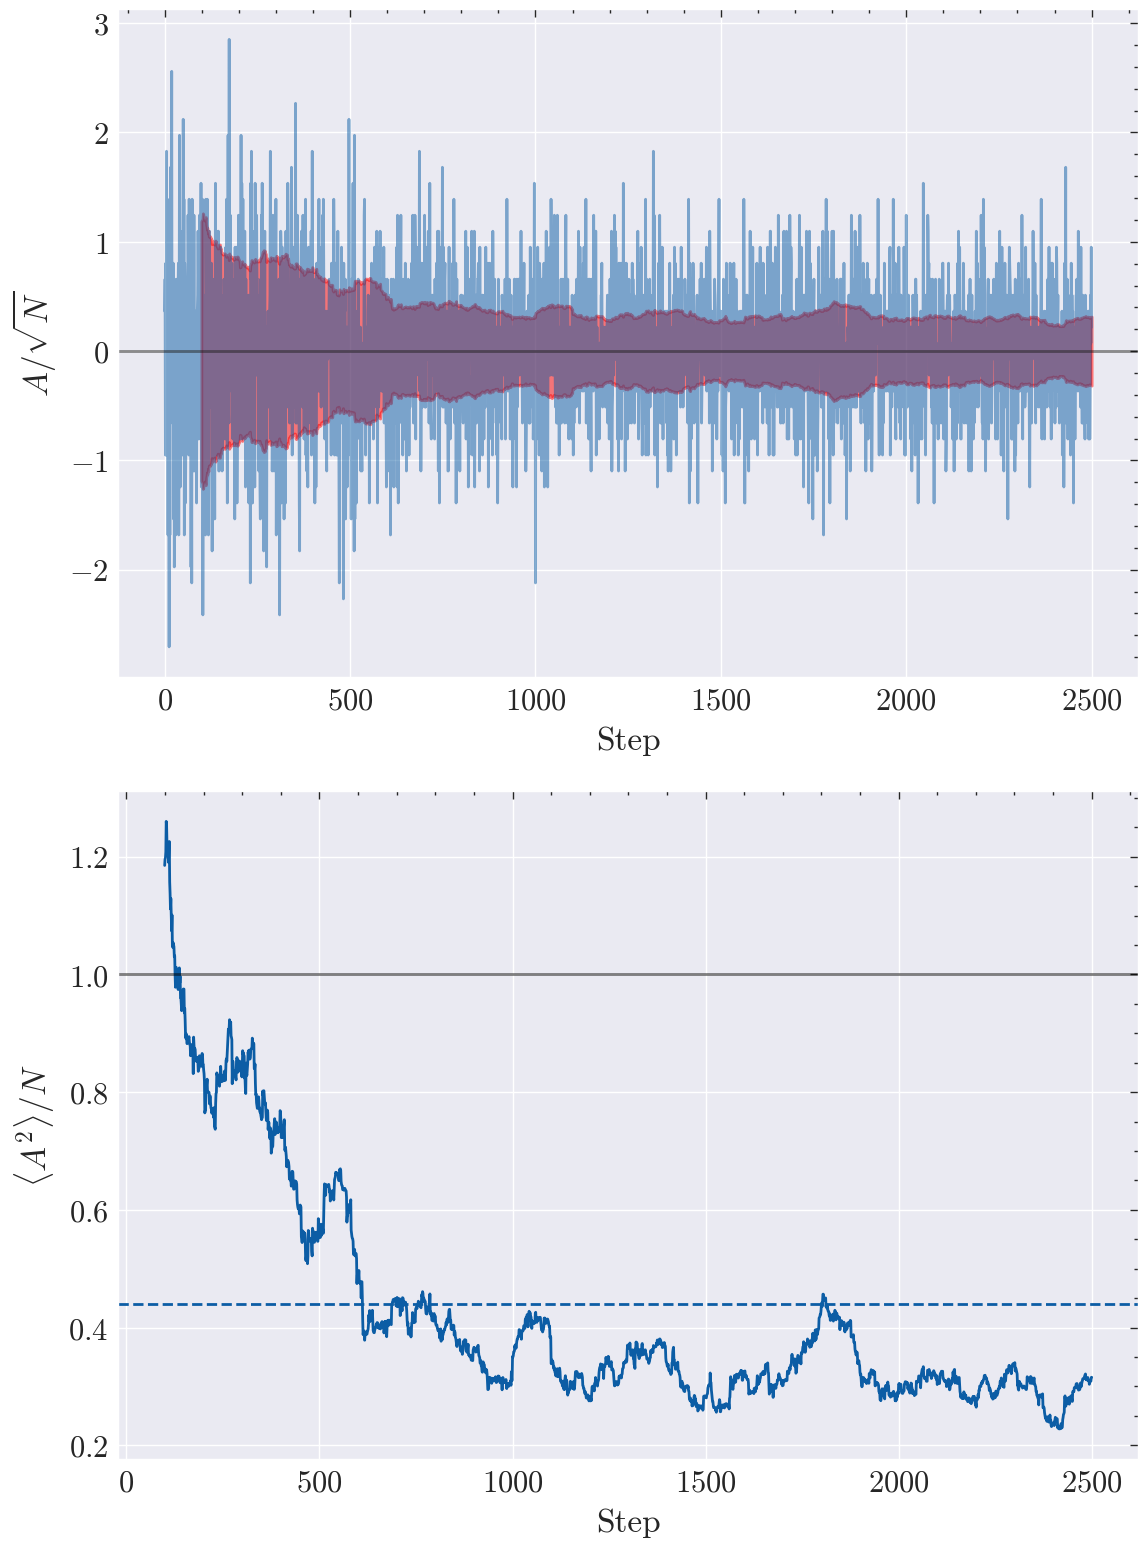
\includegraphics[width=0.42\textwidth]{figures/M6_N187.png}
    \caption{Dynamics of the system for $N=187$ and $M=6$, yielding $\alpha \simeq 0.34 \simeq \alpha_c$.}
    \label{fig:dynamics1}
\end{figure}

\begin{figure}[H]
    \centering
    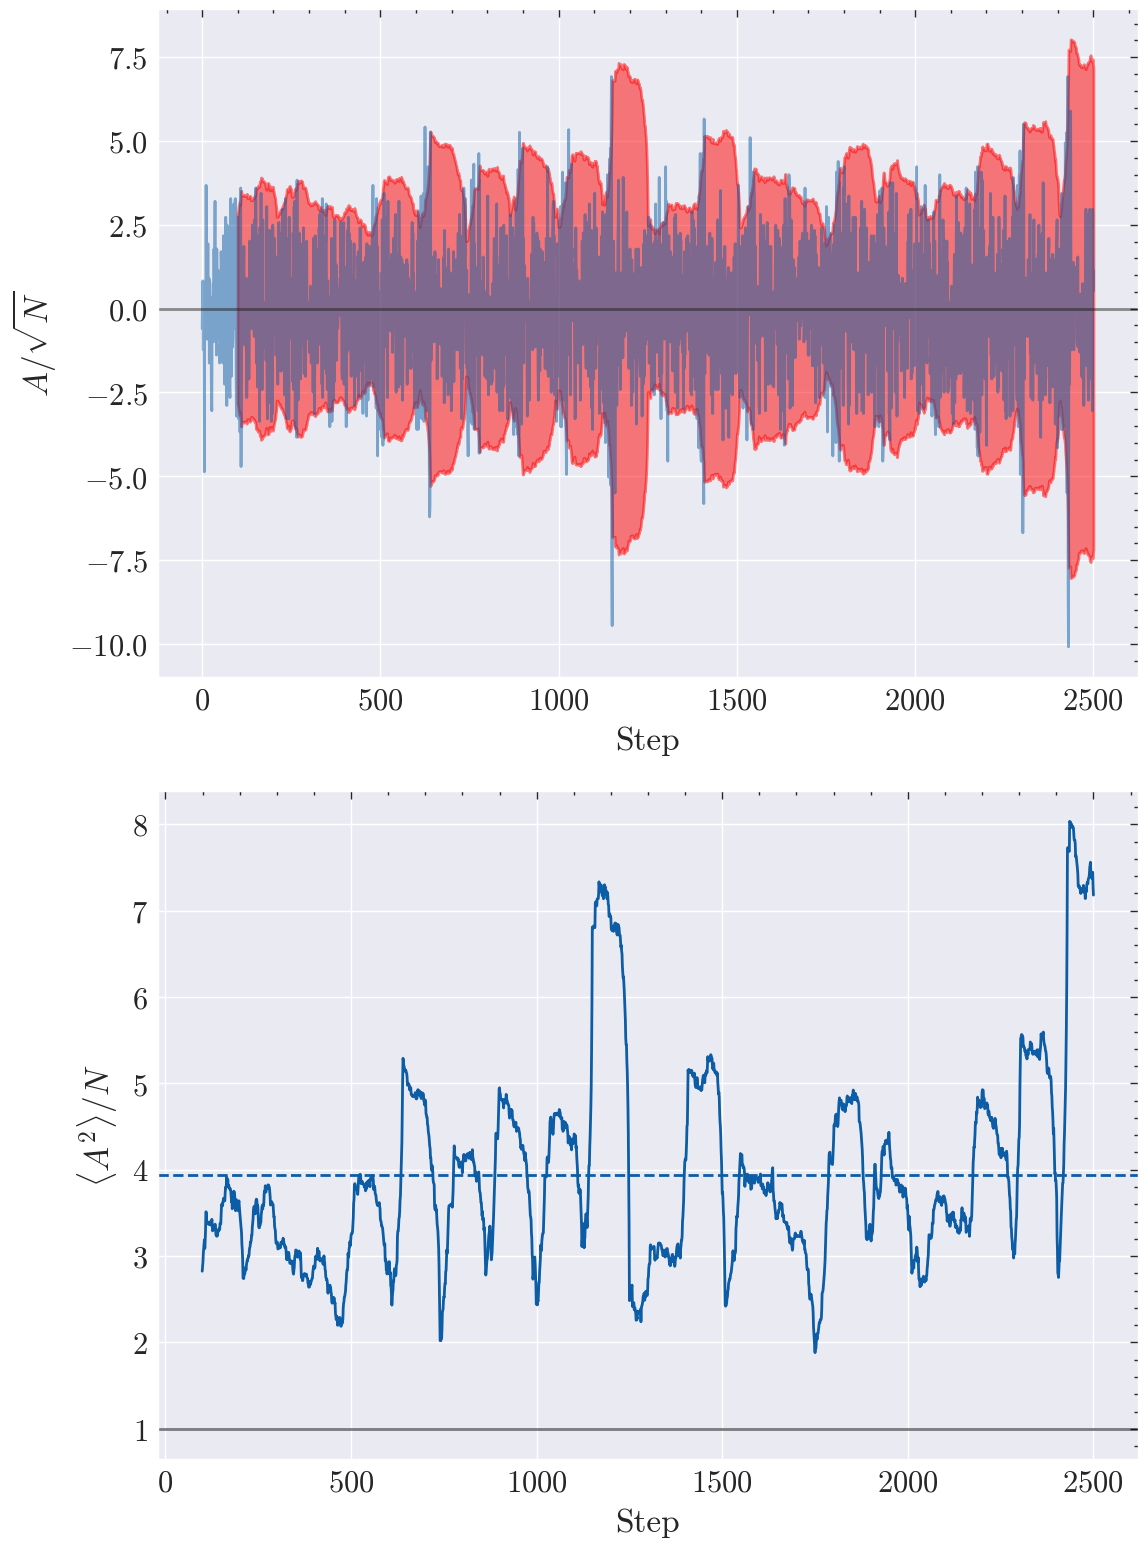
\includegraphics[width=0.42\textwidth]{figures/M6_N639.png}
    \caption{Dynamics of the system for $N=639$ and $M=6$, yielding $\alpha \simeq 0.10 \ll \alpha_c$.}
    \label{fig:dynamics2}
\end{figure}

\begin{figure}[H]
    \centering
    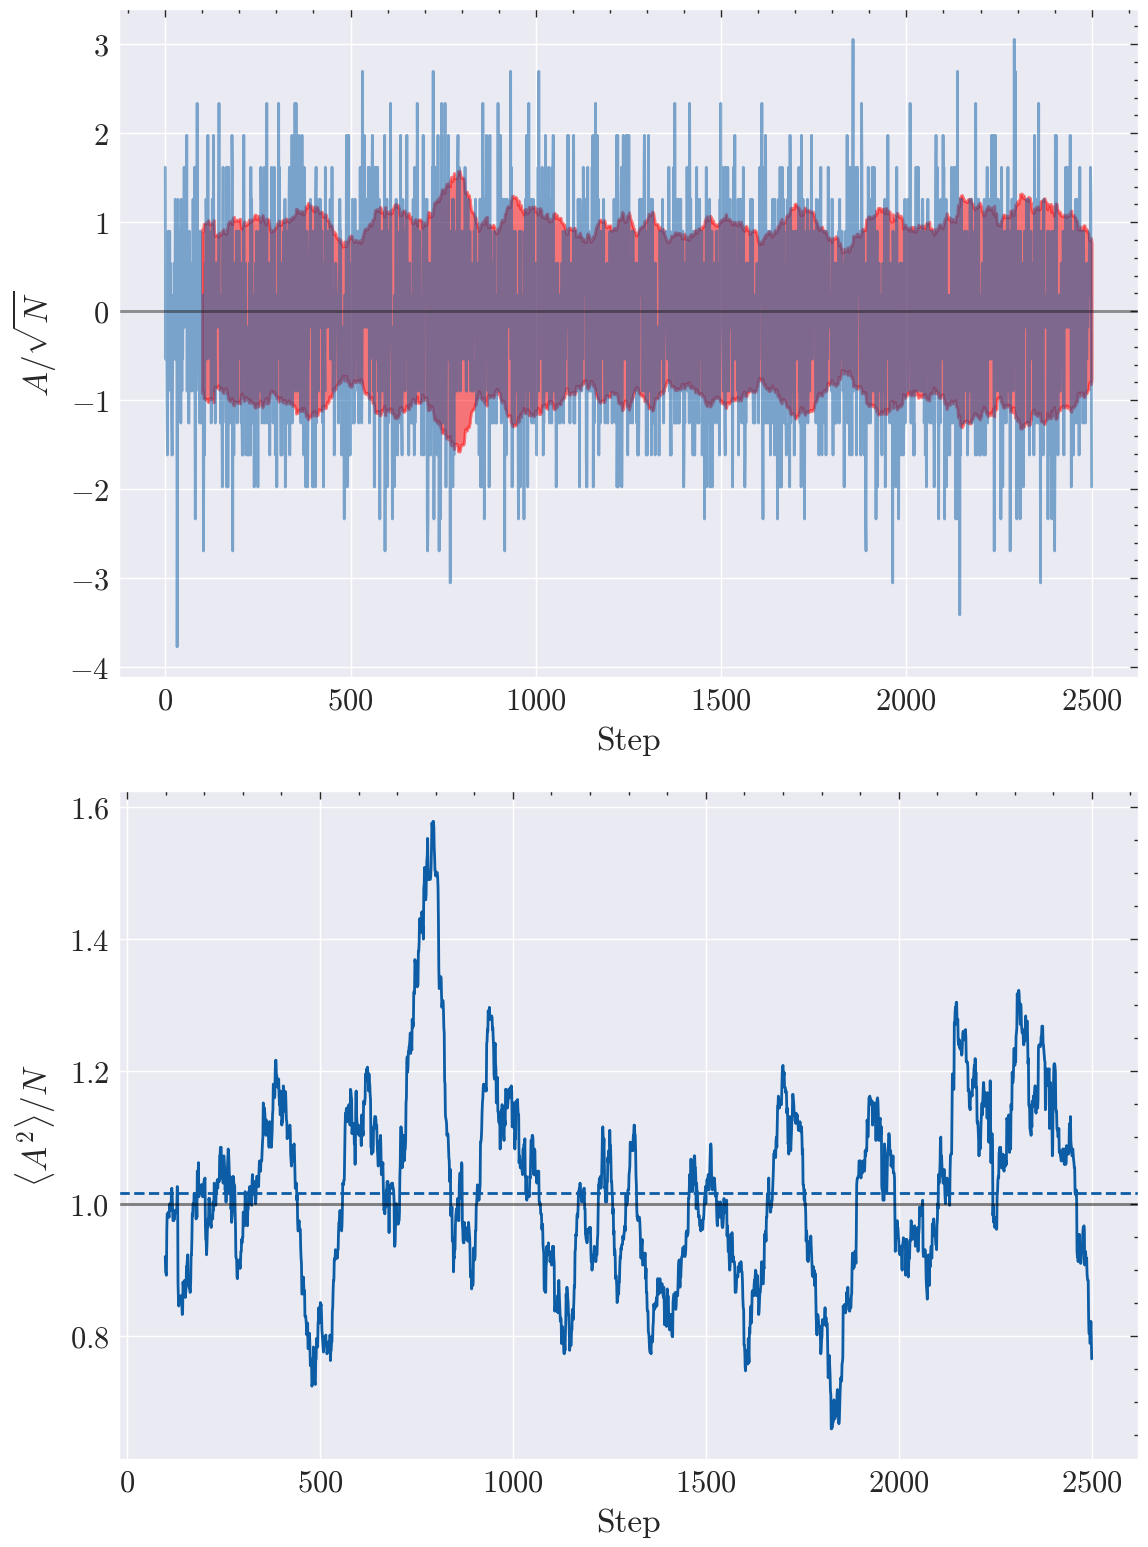
\includegraphics[width=0.42\textwidth]{figures/M10_N31.png}
    \caption{Dynamics of the system for $N=31$ and $M=10$, yielding $\alpha \simeq 33 \gg \alpha_c$.}
    \label{fig:dynamics3}
\end{figure}

Clearly, different values of $\alpha$ lead to dramatically different behaviors of the volatility of the system. To better understand the relationship between $\alpha$ and the volatility, we plot the long-term volatility of the system $\sigma^2/N$ as a function of $\alpha$ in log-log scale in Figure \ref{fig:volatility}. We can see that the system self-organizes to reduce the volatility whenever $\alpha \simeq \alpha_c$. On the contrary, when $\alpha \ll \alpha_c$, the system fails to self-organize and the volatility greatly increases to around four times the baseline volatility. Finally, when $\alpha \gg \alpha_c$, the system is still failing to self-organize, but the volatility is not worse than the baseline volatility.

In hindsight, these results can be understood as follows:
\begin{itemize}
    \item When $\alpha \ll \alpha_c$, the population is large compared to the strategy space, so we expect agents' strategies to be correlated. This correlation between agents can be thought of as a \textit{herding effect}, which explains the excess volatility and the volatility clustering.
    \item When $\alpha \gg \alpha_c$, the population is small compared to the strategy space and as such agents' strategies are likely to be uncorrelated. We escape the herding effect, but agents are now so independent that they essentially behave like \textit{random agents} flipping coins. That explains why the volatility is about the same as the baseline volatility; note that it is slightly inferior since agents aren't completely independent so they can somewhat coordinate.
    \item When $\alpha \simeq \alpha_c$, the population is about the same size as the strategy space and thus agents' strategies are correlated enough so that they can coordinate, but not so much that herding effects dominate. This is the sweet spot where the system self-organizes, reducing the volatility.
\end{itemize}

\begin{figure}[H]
    \centering
    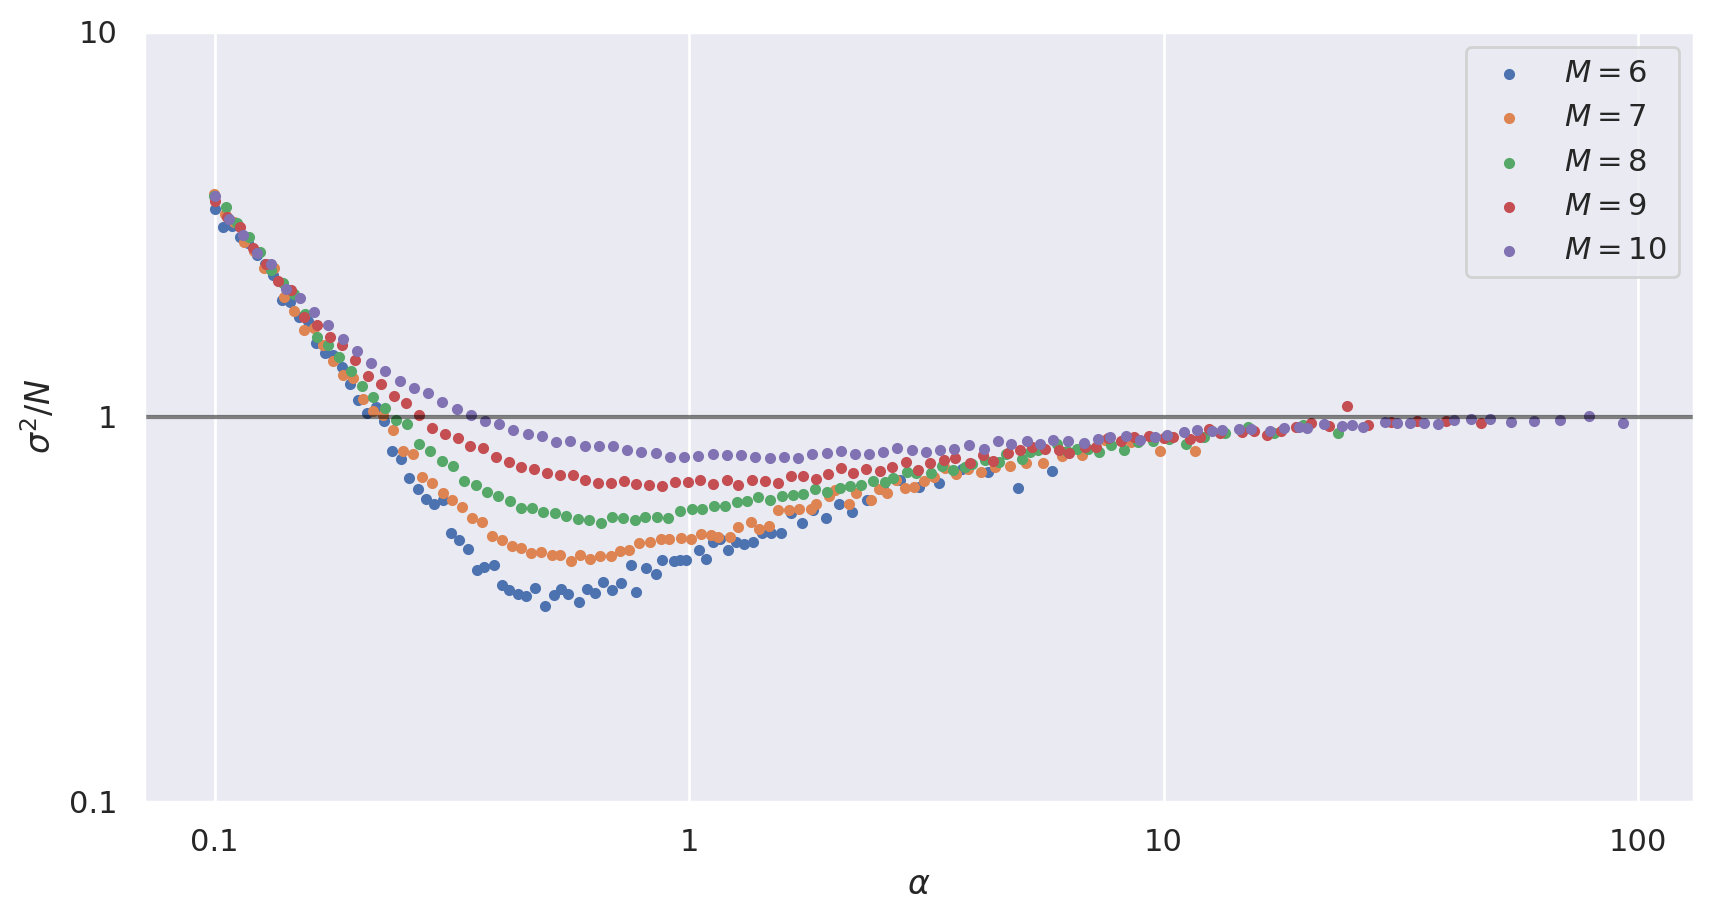
\includegraphics[width=0.42\textwidth]{figures/volatility.png}
    \caption{Long-term volatility $\sigma^2 / N$ of the system as a function of the parameter $\alpha = \frac{2^M}{N}$ for various couples $(N, M)$.}
    \label{fig:volatility}
\end{figure}

\subsection{Predictability}

Volatility is not the only quantity of interest in the Minority Game. We are also interested in the predictability of the system, which can be understood as the ability of an agent with memory $M$ to predict the attendance at time $t$. More precisely, we define the predictability $\theta^2$ of the system as:
\begin{equation}
    \theta^2 = \frac{1}{2^M} \sum_{\mu \in \{0, 1\}^M} \langle \textnormal{sign}A|\mu \rangle^2
\end{equation}

When the system is perfectly unpredictable, then $\forall \mu\in \{ 0,1\}^M \ \langle \textnormal{sign}A|\mu \rangle = 0$ i.e. knowing the past $M$ actions of the population does not help in predicting the next action of the population. On the other hand, if there are some states $\mu$ which lead to a biased outcome of the population, then $\exists \mu \ \langle \textnormal{sign}A|\mu \rangle \neq 0$ and the system has some degree of predictability. We thus have $\theta^2=0$ for fully unpredictable system and $\theta^2=1$ for a perfectly predictable system.

Again, deriving $\theta^2$ analytically is a hard problem, and we will use numerical simulations instead to study the link between $\alpha$ and the predictability of the system. The results are presented in Figure \ref{fig:predictability} where we plot the predictability $\theta^2$ of the system as a function of $\alpha$ in log scale. Here the phase transition at $\alpha_c$ is even more striking than for volatility. We observe the following two regimes:
\begin{itemize}
    \item For $\alpha < \alpha_c$, the system is unpredictable, meaning that the agents are consuming all the available information and as such there is no information left to predict the attendance.
    \item For $\alpha > \alpha_c$, $\theta^2$ increases with $\alpha$ and seems to plateau around $\theta^2 \simeq 0.4$ (though this would need more data to be confirmed). In this case, there aren't enough agents relative to the strategy space, implying that agents are not consuming all the available information. This means that there is some information left to predict the attendance, which explains the increase in predictability.
\end{itemize}
Importantly, note that although the system becomes partly predictable for $\alpha > \alpha_c$, the agents playing the game are not able to leverage this predictability to improve their performance i.e. there is no "star player". To understand why, imagine that for a certain game state $\mu_0$ the attendance is biased towards $+1$, i.e. $\langle \textnormal{sign}A|\mu_0 \rangle > 0$. Agents will quickly remark this bias will want to play $-1$ to secure a win. As more agents play $-1$, $\langle \textnormal{sign}A|\mu_0 \rangle \searrow 0$ and the anomaly disappears: by playing the edge, the agents are effectively arbitraging away the anomaly. This is due to the crucial fact that \textit{each agent has an individual impact}. Thus, the predictability that arises in the $\alpha > \alpha_c$ regime is due to anomalies that cannot be arbitraged away because there aren't enough agents to cover the whole strategy space, and as such there are "holes" in the system that no one is taking advantage of.\footnote{If we added sufficiently many agents to the system, these "holes" would be filled and the predictability would vanish. This would amount to increasing $N$ so as to decrease $\alpha$ back to the efficient phase $\alpha < \alpha_c$.}

\begin{figure}[H]
    \centering
    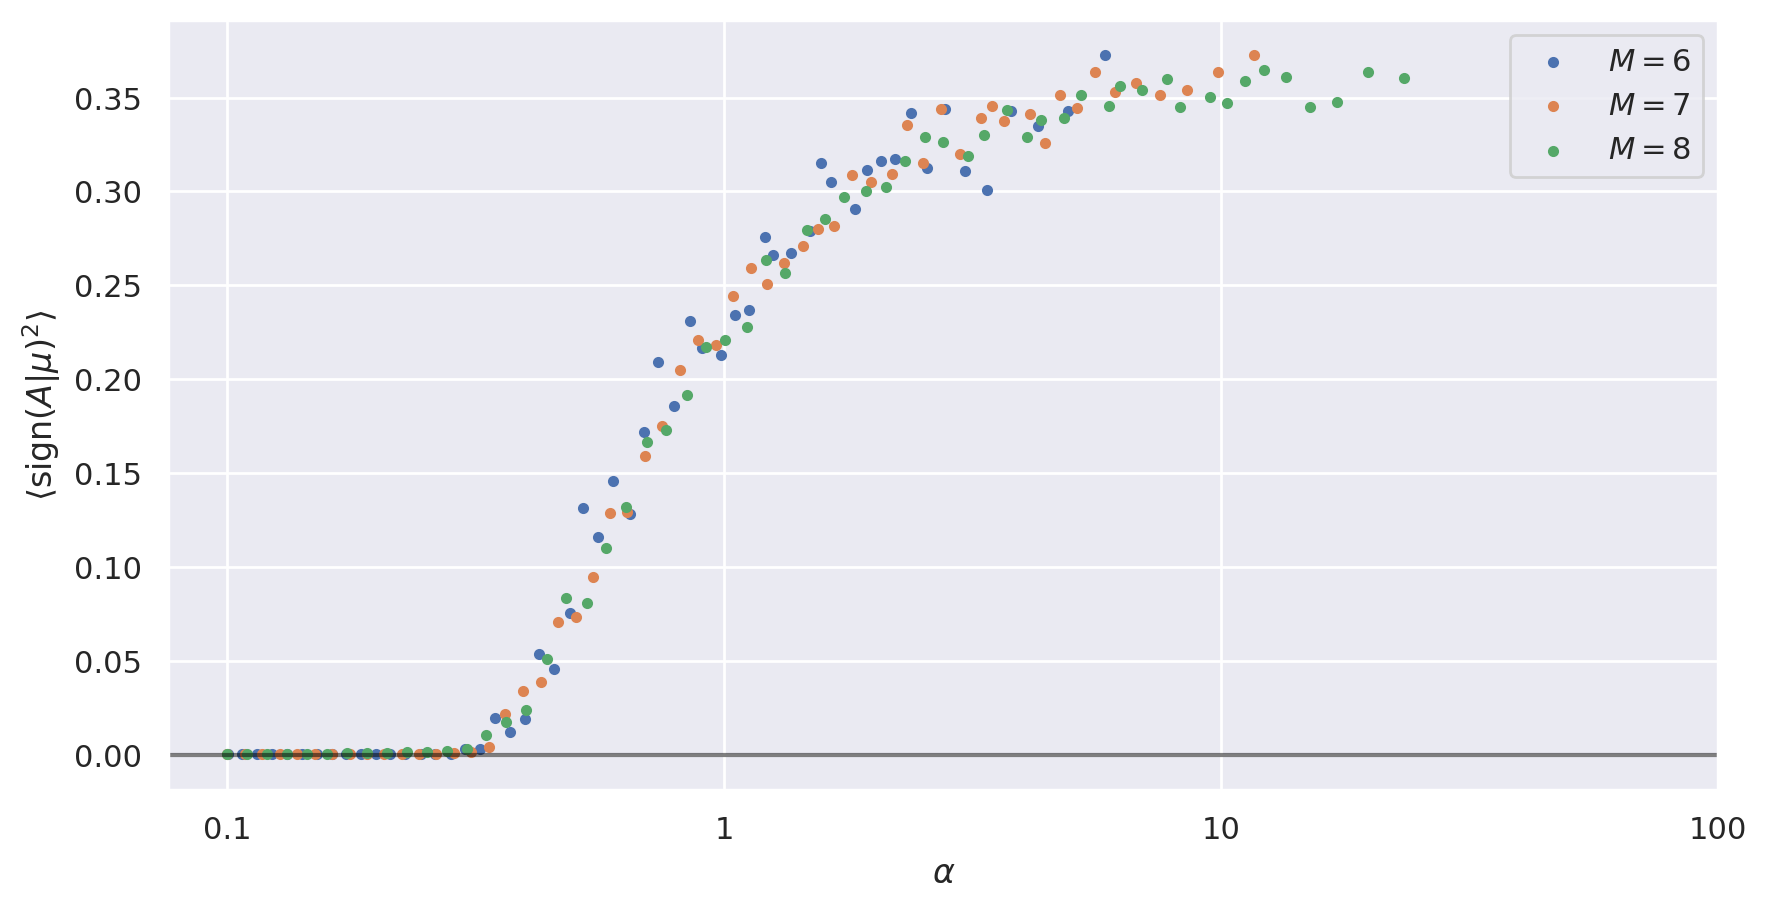
\includegraphics[width=0.42\textwidth]{figures/predictability.png}
    \caption{Predictability of the system as a function as a function of the parameter $\alpha = \frac{2^M}{N}$ for various couples $(N, M)$.}
    \label{fig:predictability}
\end{figure}


\section{Financial markets and the Minority Game}
\label{sec:financial-markets}

Given its complex volatility and predictability dynamics, it is not surprising that the Minority Game has been used to model financial markets \cite{Challet_2004}. Indeed, one can view financial markets as a collection of agents, each trying to predict the future price of an asset based on past data and using their own strategies. One can then reconsider the two identified regimes in the context of financial markets:
\begin{itemize}
    \item $\alpha < \alpha_c$ is the \textit{efficient phase} of the market, where future prices cannot be predicted and agents are correlated, leading to well-known stylized facts in the price process such as excess volatility and volatility clustering.
    \item $\alpha > \alpha_c$ is the \textit{inefficient phase} of the market, where future prices can be predicted to some extent.
\end{itemize}
Assuming the Minority Game is an acceptable first order approximation of financial markets, one may naturally wonder what value of $\alpha$ is most realistic to describe them.

To begin with, a key observation is that financial markets must remain in the efficient phase almost all the time, because as soon as they become even slightly predictable, traders will quickly step in and arbitrage away these anomalies. Arbitrageurs entering the market to correct anomalies can be interpreted in the Minority Game as an increase in the number of agents $N$ to bring the inefficient $\alpha > \alpha_c$ back to the efficient phase $\alpha < \alpha_c$.

However, going too deep into the efficient phase i.e. $\alpha \ll \alpha_c$ is also not desirable. Indeed, in this regime markets are too volatile, prompting traders to exit the market. This can be recast in the Minority Game as a decrease in the number of agents $N$ to bring $\alpha$ closer to the critical value $\alpha_c$.

As such, it seems logical that markets function near the critical value $\alpha_c$, where they are efficient enough to prevent mostly everyone to profit from them, but still offer subtle anomalous behaviors which can be exploited by the best traders. In this sense, financial markets exhibit self-organized criticality, a concept introduced by Bak, Tang and Wiesenfeld \cite{Bak_1987} to describe systems that naturally evolve towards a critical state where small perturbations can lead to large-scale events. In the context of financial markets, these large scale events are all the stylized facts we observe in the price process, such as volatility clustering, fat tails and crashes.


\bibliography{refs} % Entries are in the refs.bib file


\end{document}
